% !TEX encoding = UTF-8 Unicode
% !TEX spellcheck = en-US


% This is the root file of your thesis: thesis.tex
% A line starting with % is a comment. In some cases, I have included a command preceded by a %. You may activate the command by removing the %.

%%===================================
\documentclass[12pt]{report}
\usepackage{ramsstyle}
\usepackage{amsmath}
%%===================================
%Write the various parts of your thesis as separate files and include them into the main file by the command \include{name of included file}. When you compile the LaTeX file, you may choose which subfiles to include by the command

%\includeonly{chapter01,chapter02}

%%===================================
\begin{document}
% !TEX encoding = UTF-8 Unicode
%!TEX root = thesis.tex
% !TEX spellcheck = en-US

%This is the Titlepage
%%=========================================
\thispagestyle{empty}
%\includegraphics[scale=1.1]{fig/rams}
\mbox{}\\[6pc]
\begin{center}
\Huge{This is the Title of my Thesis}\\[2pc]

\Large{Your Name}\\[1pc]
\large{August 2014}\\[2pc]

PROJECT / MASTER THESIS\\
Department of Production and Quality Engineering\\
Norwegian University of Science and Technology
\end{center}
\vfill

\noindent Supervisor 1: Professor Ask Burlefot

\noindent Supervisor 2: Professor Fingal Olsson

 % This is the titlepage
\setcounter{page}{0}
\pagenumbering{roman}
%% !TEX encoding = UTF-8 Unicode
%!TEX root = thesis.tex
% !TEX spellcheck = en-US
%%=========================================
\addcontentsline{toc}{section}{Preface}
\section*{Preface}
Here, you give a brief introduction to your work. What it is (e.g., a Master's thesis in RAMS at NTNU as part of the study program xxx and\ldots), when it was carried out (e.g., during the autumn semester of 2021). If the project has been carried out for a company, you should mention this and also describe the cooperation with the company. You may also describe how the idea to the project was brought up.

You should also specify the assumed background of the readers of this report (who are you writing for).\\[2cm]

\begin{center}
Trondheim, 2012-12-16\\[1pc]
(Your signature)\\[1pc]
Ola Nordmann
\end{center}
%\include{acknowledgment}
%\include{summary}
%\tableofcontents
\setcounter{page}{0}
\pagenumbering{arabic}
\documentclass{article}
\usepackage{amsmath}
\usepackage{bm}
\usepackage{graphicx}
\usepackage[utf8]{inputenc}
\usepackage{caption}
\usepackage{subcaption}
\title{Modeling a synaptic transmission, \\
Mathematical modeling}
\author{Student numbers }


\begin{document}
\maketitle


\section{Introduction}
%We chose project 1. Our focus was making numerical solvers for the problem in all dimensions, and putting som boundary conditions on the edges to estimate the time for the signalt to transmitt. We also modeled the time using what we have learned for matematical modeling. \\
We tried to find the time estimate for the signal to be transmitted in several different ways. 
A good way to start was by finding a time 	scale. 


In this report, we start by showing a Monte Carlo simulation of random walk as a first model for the diffusion of the neurotransmitters.  Next, modeling equations are derived for the initial model, as well as the expanded model which includes the glia cells.  After this, mathematical modeling is used to obtain a rough estimate of the time used to transmit a signal. This is followed by several attempts at solving a 1D model of the problem, and then a 2D model.



\begin{thebibliography}{9}
%\cite[p. 34]{holstad}%
\bibitem{holstad}
  Jörg Henrik Holstad,
  \emph{Modellering av Diffusjon av Nevrotransmittere
i den Ekstracellulære Væsken}.
  2011.\\
https://www.duo.uio.no/bitstream/handle/10852/10871/MasteroppgaveHenrikHolstad.pdf
Retrieved 13.11.2014
\end{thebibliography}
\end{document}
\section{Modeling a time scale}
We wanted to find a scaling for time in order to get a feel about the time it takes before a signal is transmitted. In order to do that, we use the diffusion equation
\begin{align}
\label{diffusion_unscaled}
\frac{\partial c^{*}}{\partial t^{*}} = \kappa \nabla^2 c^{*}.
\end{align}
Since we were given a radius and a height, we chose to use cylindrical coordinates. Thus $\nabla^2$ becomes
$$ \nabla^2 f = \frac{1}{r^{*}} \frac{\partial}{\partial r^{*}} \Big( r^{*} \frac{\partial f}{\partial r^{*}} \Big) +\frac{1}{(r^{*})^2}\frac{\partial^2 f}{\partial \phi^2} + \frac{\partial^2 f}{\partial (z^{*})^2}. $$
We scale the equation so that
$$\begin{array}{lr}
c^{*} &= Cc\\ r^{*} &=Rr\\ z^{*} &= Lz\\ t^* &=Tt.\\
\end{array}$$
With the scaling, the equation becomes
$$\frac{\partial Cc}{\partial Tt} = \kappa \Bigg( \frac{1}{Rr} \frac{\partial }{\partial Rr} \Big( Rr \frac{\partial Cc}{\partial Rr} \Big) +\frac{1}{(Rr)^2}\frac{\partial^2 Cc}{\partial \phi^2} + \frac{\partial^2 Cc}{\partial (Lz)^2} \Bigg). $$
We assume that the neurotransmitters are released in the centre of the axon. Due to rotational symmetry, $c$ becomes independent of $\phi$. Since $R >> h$, it follows that $1/R^2<<1/L^2$, and we assume $1/R^2 \approx 0$. After these simplifications the equation becomes
$$\frac{1}{T} \frac{\partial c}{\partial t} = \kappa  \frac{1}{L^2}\frac{\partial^2 c}{\partial z^2} . $$
To simplify, we set all derivatives to be $ \sim 1 $, and obtain
$$\frac{1}{T}  = \kappa \frac{1}{L^2}.  $$
Solving for $T$ gives us a timescale
$$T = \frac{L^2}{\kappa} = \frac{(15\cdot 10^{-9}\text{m})^2}{0.3\cdot 10^{-12} \text{m$^2$/s}} = 0.75 \text{ms}. $$
This is by no means a correct time for the signal to be transmitted, but we could guess that the real time will be of order $1 \text{ms}$.
\section{2D diffusion equation}

\subsubsection{Domain, initial and boundary values}

Initially we chose a random point where we released all the neurotransmitters. The initial function for the concentration of neurotransmitters is zero everywhere except from that point. On the boundary we assumed that the particles could freely diffuse outside of the domain.\\
To simplify the diffusion equation we neglect the height of the synaptic cleft. Furthermore, we chose to view the resulting disc as a square with size $4r^2$, due to the difficut nature of the laplacian in cylindrical coordinates. We assume that the receptors are equally distributed over the square.\\If the number of bounded receptor doesn't change over a time interval $\Delta t$, we assume equilibrium and that a signal is being transmitted. \\


\subsubsection{Numerical scheme}
We used the finite difference method to discretize the modelling equations. OBS!(ref.)
$$c_{j,k}^{i+1}=c_{j,k}^{i}+\frac{\Delta t}{2} \Bigg[\kappa \Big(\frac{c_{j+1,k}^{i} -2c_{j,k}^{i} + c_{j-1,k}^{i}}{(\Delta y)^2} +\frac{c_{j,k+1}^{i} -2c_{j,k}^{i} + c_{j,k-1}^{i}}{(\Delta x)^2}\Big)-k_{1}c_{j,k}^i P_{j,k}^i+k_{2}(1-P_{j,k}^i)\Bigg]$$

$$P_{j,k}^{i+1}=P_{j,k}^i + \Delta t \Big[-k_{1}c_{j,k}^iP_{j,k}^i+k_{2}(1-P_{j,k}^i) \Big]$$

\subsubsection{Results}
Using the values given in \cite{fg} with $k_1=10^4$ and $k_2=10$, and 
\begin{itemize}
\item number of steps in x- and y-direction, $nx=ny=10$
\item number of time steps $nt=4\cdot 10^5$, simulated over 1 second
\end{itemize}
This results in a signaling time of $t_s=33.8$ms. The following figures shows the distribution of neurotransmittors and free receptors at the signaling time. 

%results\\
%\begin{figure}
%\begin{subfigure}[b]
%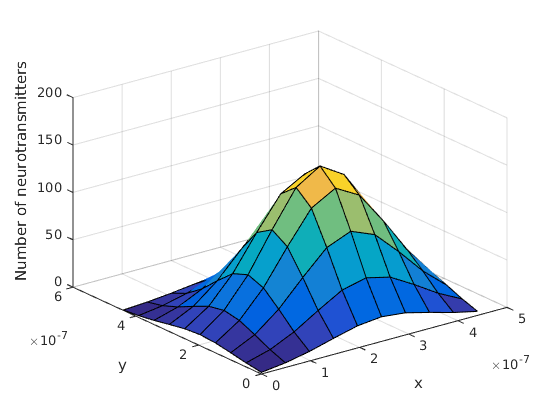
\includegraphics[scale=0.25]{distneurottansmitters}
%\caption{yolo}
%\end{subfigure}
%\begin{subfigure}[b]
%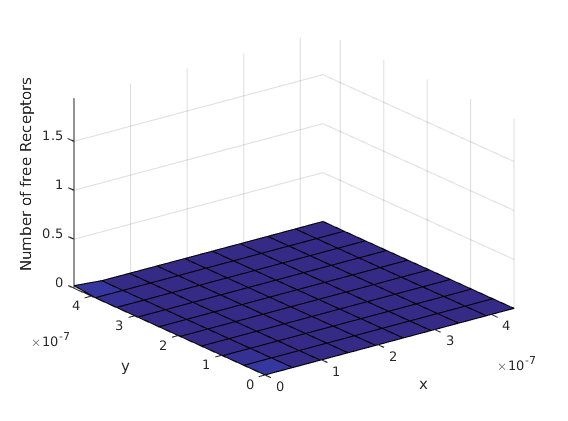
\includegraphics[scale=0.25]{receptordensity}
%\caption{tt}
%\end{subfigure}
%\end{figure}
%
%\begin{figure*}[h!]
%    \centering
%    \begin{subfigure}[b]{0.5\textwidth}
%        \centering
%        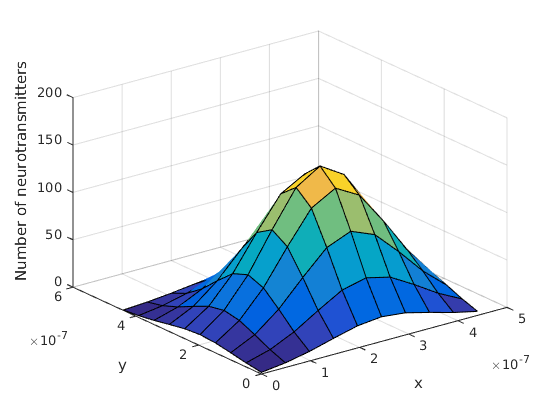
\includegraphics[height=1.2in]{distneurottansmitters}
%        \caption{Neurotransmitters}
%    \end{subfigure}%
%    ~ 
%    \begin{subfigure}[b]{0.5\textwidth}
%        \centering
%        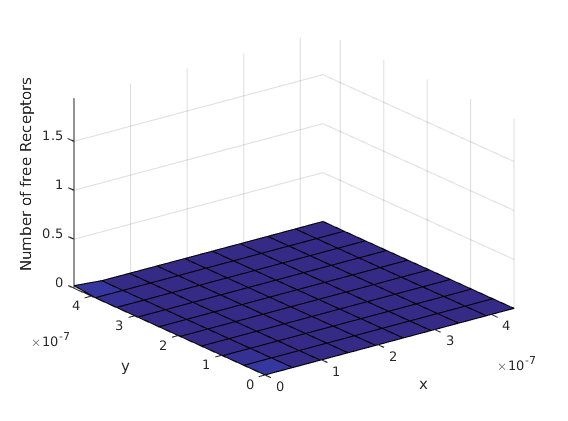
\includegraphics[height=1.2in]{receptordensity}
%        \caption{Receptors}
%    \end{subfigure}
%    \caption{Distribution after a time t=.}
%\end{figure*}


\begin{figure*}[h!]
    \centering
    \begin{subfigure}[b]{0.5\textwidth}
        \centering
        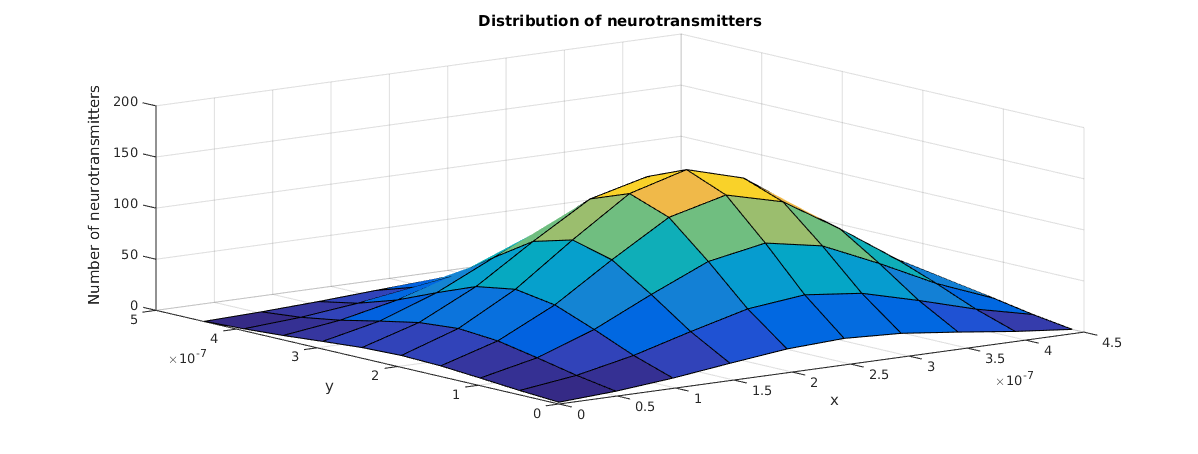
\includegraphics[scale=0.25]{1}
        \caption{Neurotransmitters}
    \end{subfigure}%
    ~ 
    \begin{subfigure}[b]{0.5\textwidth}
        \centering
        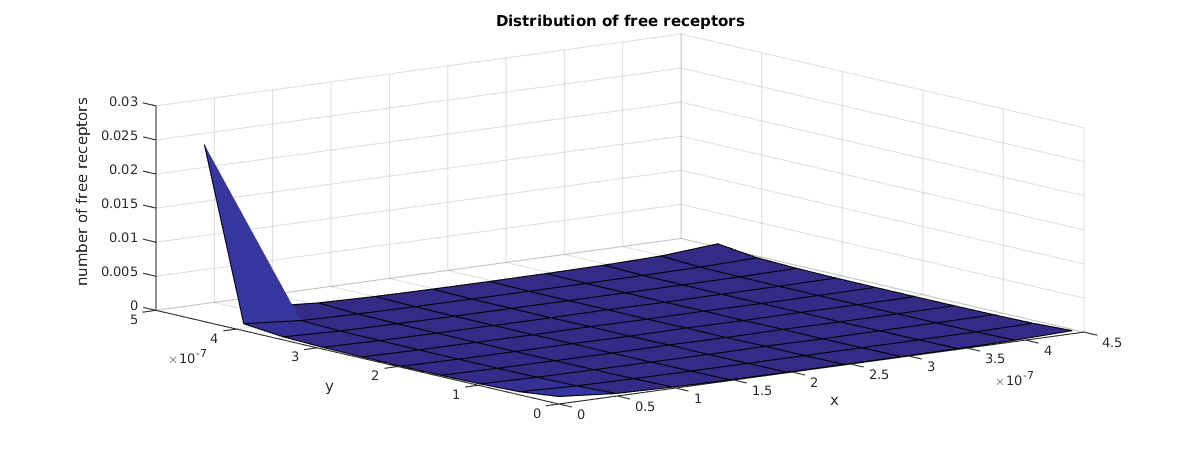
\includegraphics[scale=0.25]{2}
        \caption{Receptors}
        \label{fig1}
    \end{subfigure}
    \caption{Distribution at signal time.}
\end{figure*}

\subsubsection{Discussion}
As we can see from figure \ref{fig1} practically all receptors are bounded at this time, so this may be considered an upper bound for the signaling time. This is a two dimensional model, and thus lacs a certain accuracy. Given more time the model could have been extended to three dimensions, but as a simple representation of what happens during neurotransmission in the synaptic cleft, we consider this model is applicable.\\ Given more time, this model could also have been used to model the clearance time.
% Include more chapters as required.
%%=========================================
%\appendix
%\include{acronyms}
%\include{appendix-b}
% Include more appendices as required.
%%=========================================
%\bibliographystyle{apa}
%\addcontentsline{toc}{chapter}{\bibname}
%\bibliography{refs}  
%%=========================================
%\include{vitae}         % Your curriculum Vitae     
%%=============================================

\end{document}
